\documentclass[tikz,border=8pt]{standalone}
\usepackage[T1]{fontenc}
\usepackage{helvet}
\renewcommand{\familydefault}{\sfdefault}
\usepackage{amsmath}
\usepackage{xcolor}
\usetikzlibrary{arrows.meta, positioning}

\definecolor{ink}{HTML}{1F2937}
\definecolor{blueB}{HTML}{2F6B9A}
\definecolor{tealB}{HTML}{1D8B74}
\definecolor{orangeB}{HTML}{C86A1A}
\definecolor{grayB}{HTML}{5B6470}
\definecolor{greenA}{HTML}{EAF7E9}
\definecolor{greenB}{HTML}{2E7D32}
\definecolor{redA}{HTML}{FDECEC}
\definecolor{redB}{HTML}{B23A3A}
\definecolor{panel}{HTML}{F8FAFC}

\tikzset{
  title/.style={font=\bfseries\fontsize{24}{26}\selectfont, text=ink},
  subtitle/.style={font=\bfseries\fontsize{15}{17}\selectfont, text=ink},
  body/.style={font=\fontsize{11}{13}\selectfont, text=ink},
  smallbody/.style={font=\fontsize{10}{12}\selectfont, text=ink},
  box/.style={rounded corners=14pt, draw=grayB!35, line width=1.1pt, fill=panel, inner sep=12pt, align=left}
}
\newcommand{\subtitle}{\bfseries\fontsize{15}{17}\selectfont\color{ink}}
\newcommand{\body}{\fontsize{11}{13}\selectfont\color{ink}}
\newcommand{\smallbody}{\fontsize{10}{12}\selectfont\color{ink}}

\begin{document}
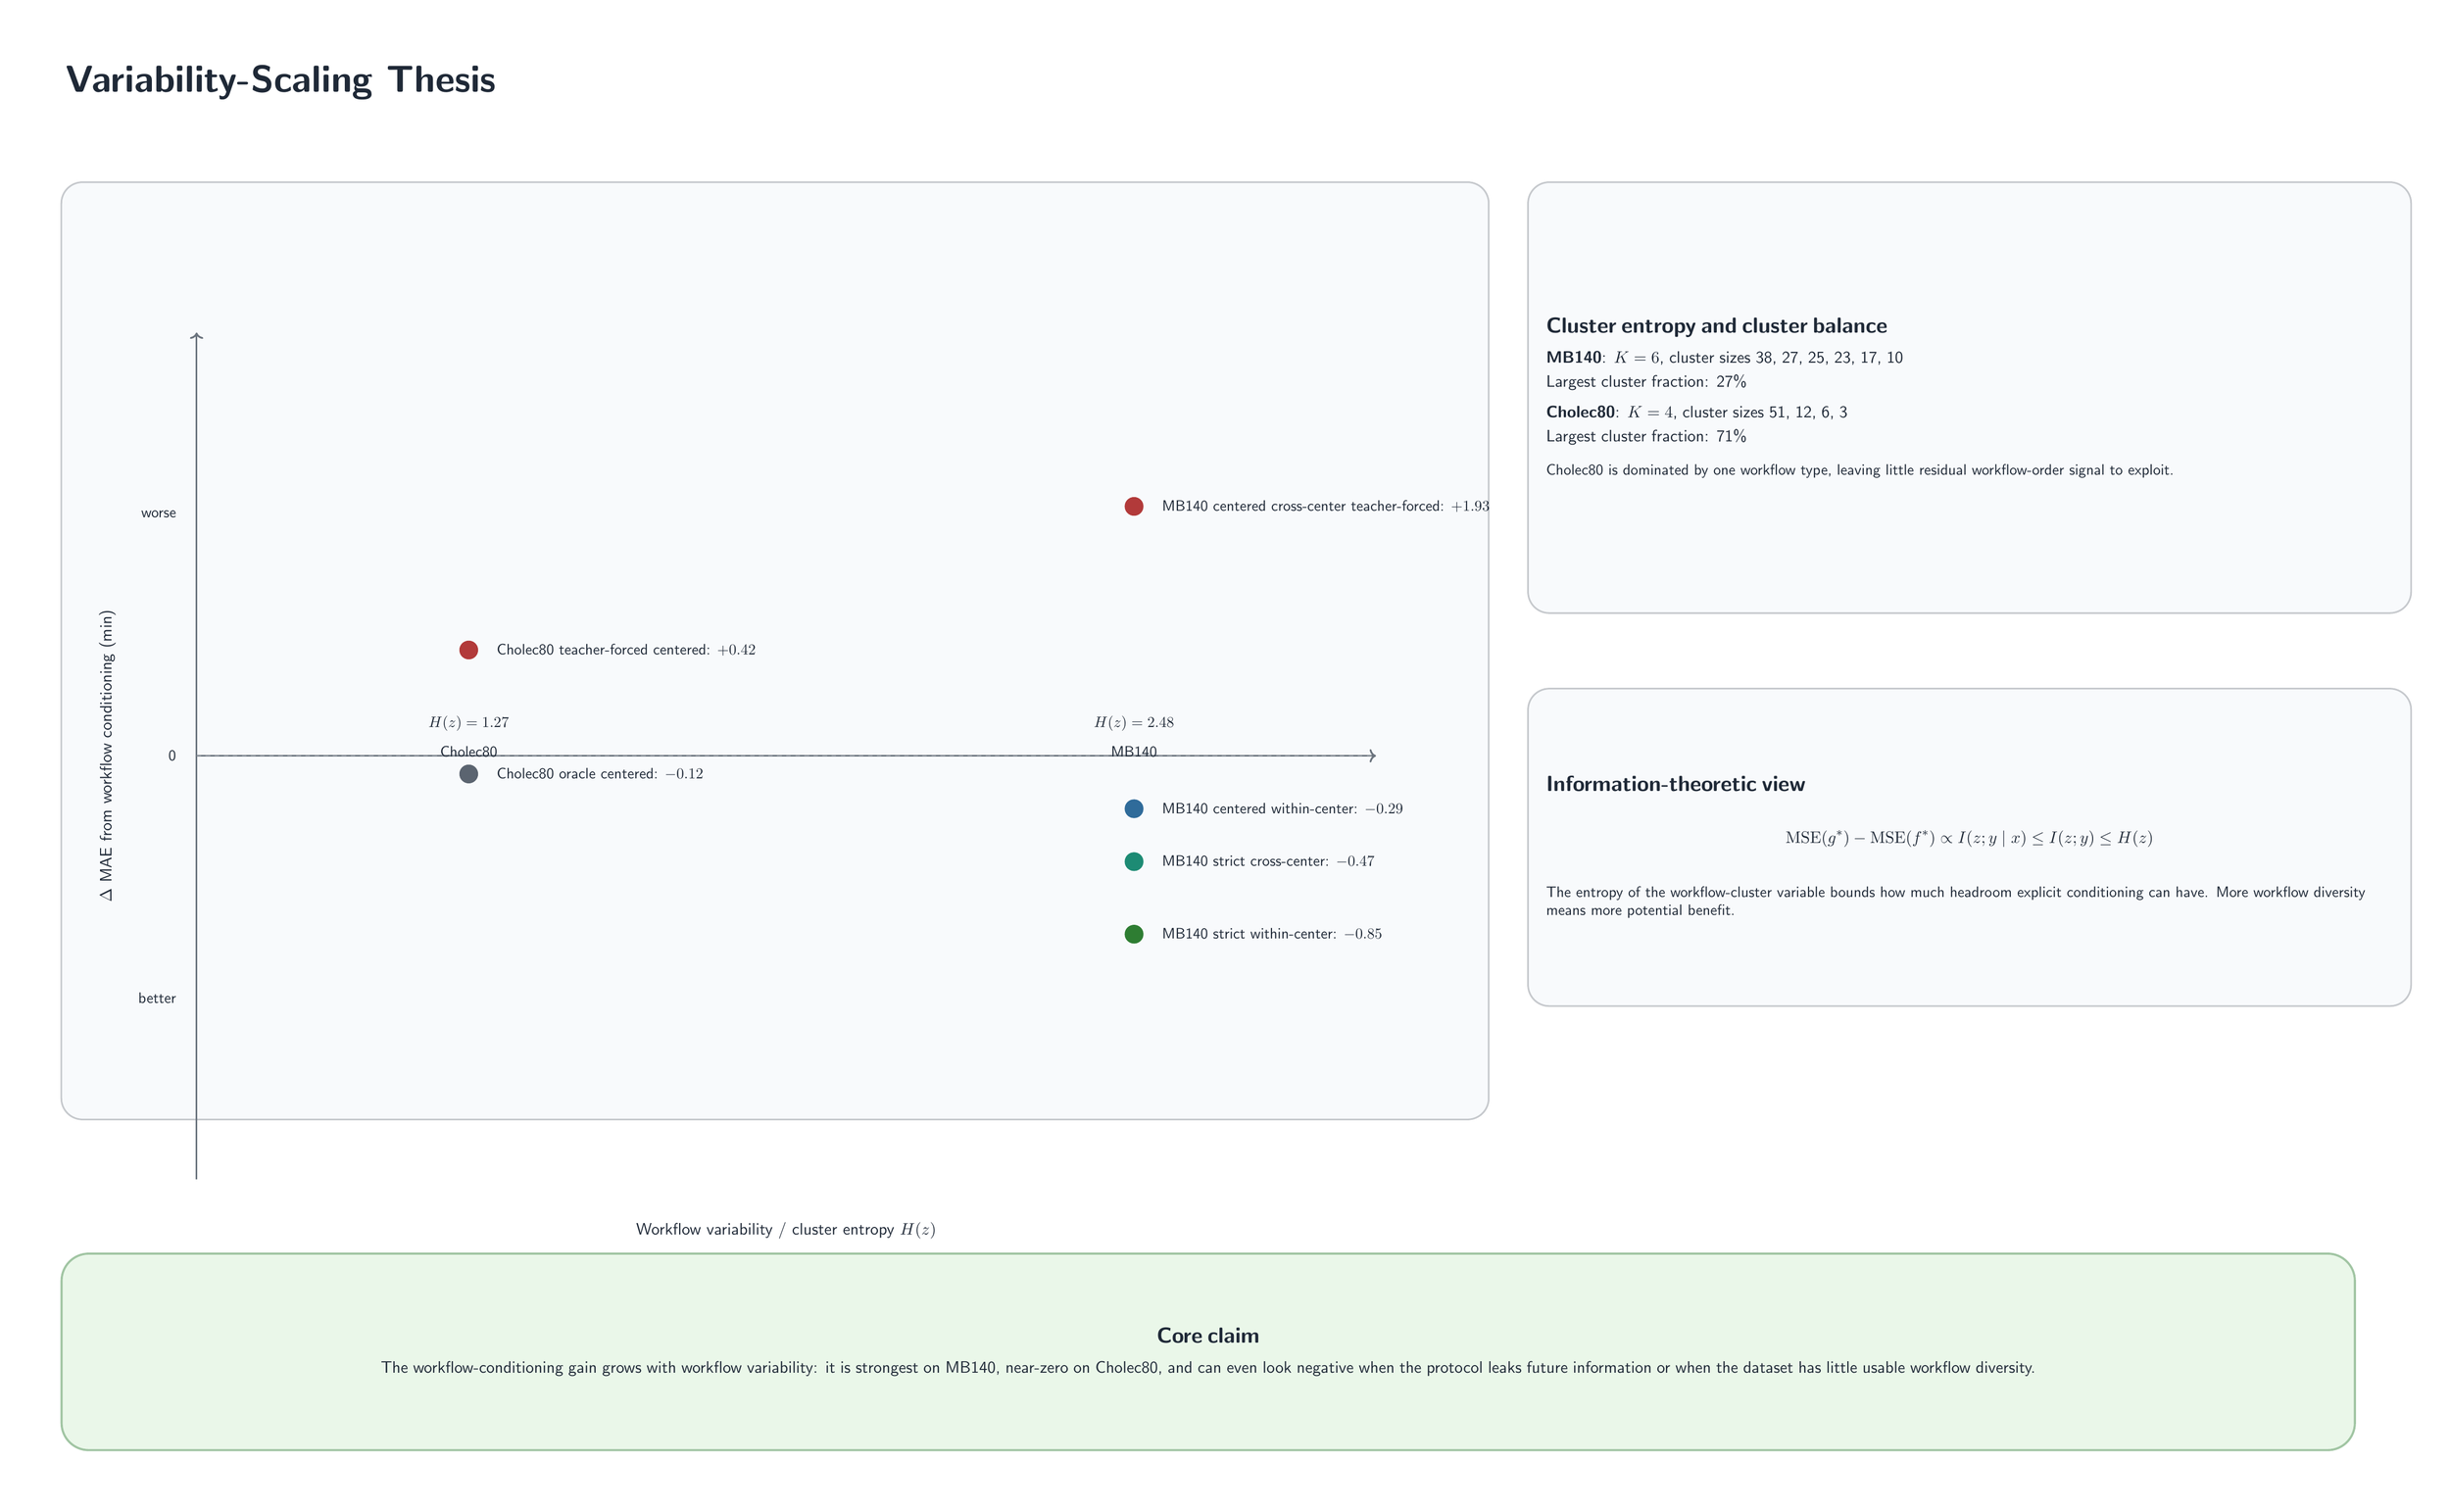
\begin{tikzpicture}[x=1pt,y=1pt]
\useasboundingbox (0,0) rectangle (1600,980);

\node[title, anchor=north west] at (30,950)
{Variability-Scaling Thesis};

\node[box, text width=920pt, minimum height=620pt, anchor=north west] at (30,870) {};

\draw[->, line width=1.2pt, color=grayB!90] (120,210) -- (120,770);
\draw[->, line width=1.2pt, color=grayB!90] (120,490) -- (900,490);
\node[rotate=90, anchor=south, body] at (70,490) {$\Delta$ MAE from workflow conditioning (min)};
\node[anchor=north, body] at (510,185) {Workflow variability / cluster entropy \(H(z)\)};

\draw[dashed, color=grayB!50] (120,490) -- (900,490);
\node[smallbody, anchor=east] at (110,490) {0};
\node[smallbody, anchor=east] at (110,650) {worse};
\node[smallbody, anchor=east] at (110,330) {better};

\node[smallbody, anchor=north] at (300,500) {Cholec80};
\node[smallbody, anchor=north] at (740,500) {MB140};
\node[smallbody, anchor=north] at (300,520) {\(H(z)=1.27\)};
\node[smallbody, anchor=north] at (740,520) {\(H(z)=2.48\)};

\filldraw[fill=greenB, draw=greenB] (740,372) circle (6pt);
\node[smallbody, anchor=west] at (755,372) {MB140 strict within-center: \(-0.85\)};

\filldraw[fill=tealB, draw=tealB] (740,420) circle (6pt);
\node[smallbody, anchor=west] at (755,420) {MB140 strict cross-center: \(-0.47\)};

\filldraw[fill=blueB, draw=blueB] (740,455) circle (6pt);
\node[smallbody, anchor=west] at (755,455) {MB140 centered within-center: \(-0.29\)};

\filldraw[fill=redB, draw=redB] (740,655) circle (6pt);
\node[smallbody, anchor=west] at (755,655) {MB140 centered cross-center teacher-forced: \(+1.93\)};

\filldraw[fill=grayB, draw=grayB] (300,478) circle (6pt);
\node[smallbody, anchor=west] at (315,478) {Cholec80 oracle centered: \(-0.12\)};

\filldraw[fill=redB, draw=redB] (300,560) circle (6pt);
\node[smallbody, anchor=west] at (315,560) {Cholec80 teacher-forced centered: \(+0.42\)};

\node[box, text width=560pt, minimum height=285pt, anchor=north west] at (1000,870) {
{\subtitle Cluster entropy and cluster balance}\par\vspace{8pt}
{\body \textbf{MB140}: \(K=6\), cluster sizes 38, 27, 25, 23, 17, 10}\par\vspace{4pt}
{\body Largest cluster fraction: 27\%}\par\vspace{8pt}
{\body \textbf{Cholec80}: \(K=4\), cluster sizes 51, 12, 6, 3}\par\vspace{4pt}
{\body Largest cluster fraction: 71\%}\par\vspace{10pt}
{\smallbody Cholec80 is dominated by one workflow type, leaving little residual workflow-order signal to exploit.}
};

\node[box, text width=560pt, minimum height=210pt, anchor=north west] at (1000,535) {
{\subtitle Information-theoretic view}\par\vspace{8pt}
{\body \[
\mathrm{MSE}(g^*)-\mathrm{MSE}(f^*) \propto I(z;y \mid x) \le I(z;y) \le H(z)
\]}\par\vspace{6pt}
{\smallbody The entropy of the workflow-cluster variable bounds how much headroom explicit conditioning can have. More workflow diversity means more potential benefit.}
};

\node[rounded corners=18pt, draw=greenB!45, fill=greenA, line width=1.4pt, text width=1510pt, minimum height=130pt, align=center, anchor=south west] at (30,30) {
{\subtitle Core claim}\par\vspace{8pt}
{\body The workflow-conditioning gain grows with workflow variability: it is strongest on MB140, near-zero on Cholec80, and can even look negative when the protocol leaks future information or when the dataset has little usable workflow diversity.}
};

\end{tikzpicture}
\end{document}
